%
%
\documentclass[twoside,11pt]{../sty/report_petsc}

\usepackage{makeidx,xspace}
\usepackage[bookmarksopen,colorlinks]{hyperref}
\usepackage[all]{hypcap}
\usepackage{color}
\input pdfcolor.tex

\usepackage[pdftex]{graphicx}


\usepackage{times}
\usepackage{listings}
\usepackage{tikz}
%\usepackage{psfig}
\usepackage{../sty/verbatim}
\usepackage{../sty/tpage}
\usepackage{../sty/here}
\usepackage{../sty/anlhelper}
\usepackage[hyphens,spaces,obeyspaces]{../sty/trl}

\setlength{\textwidth}{6.5in}
\setlength{\oddsidemargin}{0.0in}
\setlength{\evensidemargin}{0.0in}
\setlength{\textheight}{9.2in}
\setlength{\topmargin}{-.8in}

\newcommand{\findex}[1]{\index{#1}}
\newcommand{\sindex}[1]{\index{#1}}
\newcommand{\A}{\mbox{\boldmath \(A\)}}
\newcommand{\F}{\mbox{\boldmath \(F\)}}
\newcommand{\J}{\mbox{\boldmath \(J\)}}
\newcommand{\x}{\mbox{\boldmath \(x\)}}
\newcommand{\bb}{\mbox{\boldmath \(b\)}}
\newcommand{\rr}{\mbox{\boldmath \(r\)}}
hyperbaseurl

\makeindex

% Defines the environment where design issues are discussed. In the manual
% version of this report, these regions are ignored.
\def\design{\medskip \noindent Design Issue:\begin{em}}
\def\enddesign{\end{em} \medskip}
% Manual version:
% \def\design{\comment}
% \def\enddesign{\endcomment}

% Print DRAFT in large letters across every page
%\special{!userdict begin /bop-hook{gsave 200 70 translate
%65 rotate /Times-Roman findfont 216 scalefont setfont
%0 0 moveto 0.95 setgray (DRAFT) show grestore}def end}

% Defines that we're doing the whole manual, not the short intro part,
% used in part1.tex.
\def\shortintro{false}

\usepackage{fancyhdr,lastpage}
\pagestyle{fancy}
\rhead{PETSc 3.6 \today}

\begin{document}


%%%%%%%%%%%%%%%%%%%%%%%%%%%%%%%%%%%%%%%%%%%%%%%%%%%%%%%%%%%%%%%%%%%%%%%%%%%%%%%%%%%%

\pagestyle{empty}
\hspace{-.65in}
\includegraphics{ArgonneLogo}
\hfill  {\large {\bf ANL-95/11 Rev 3.6}}

\vspace*{3in}
\noindent {\huge{\bf PETSc Users Manual}}
\vspace*{8pt}
\hrule
\vspace*{8pt}
\noindent {\Large{\it Revision 3.6}}

\vspace*{1in}
\noindent \\
{\Large {\bf Mathematics and Computer Science Division}}

\vspace*{10pt}


\vspace*{20pt}


%%%%%%%%%%%%%%%%%%%%%%%%%%%%%%%%%%%%%%%%%%%%%%%%%%%%%%%%%%%%%%%%%%%%%%%%%%%%%%%%%%%%

\newpage
\centerline{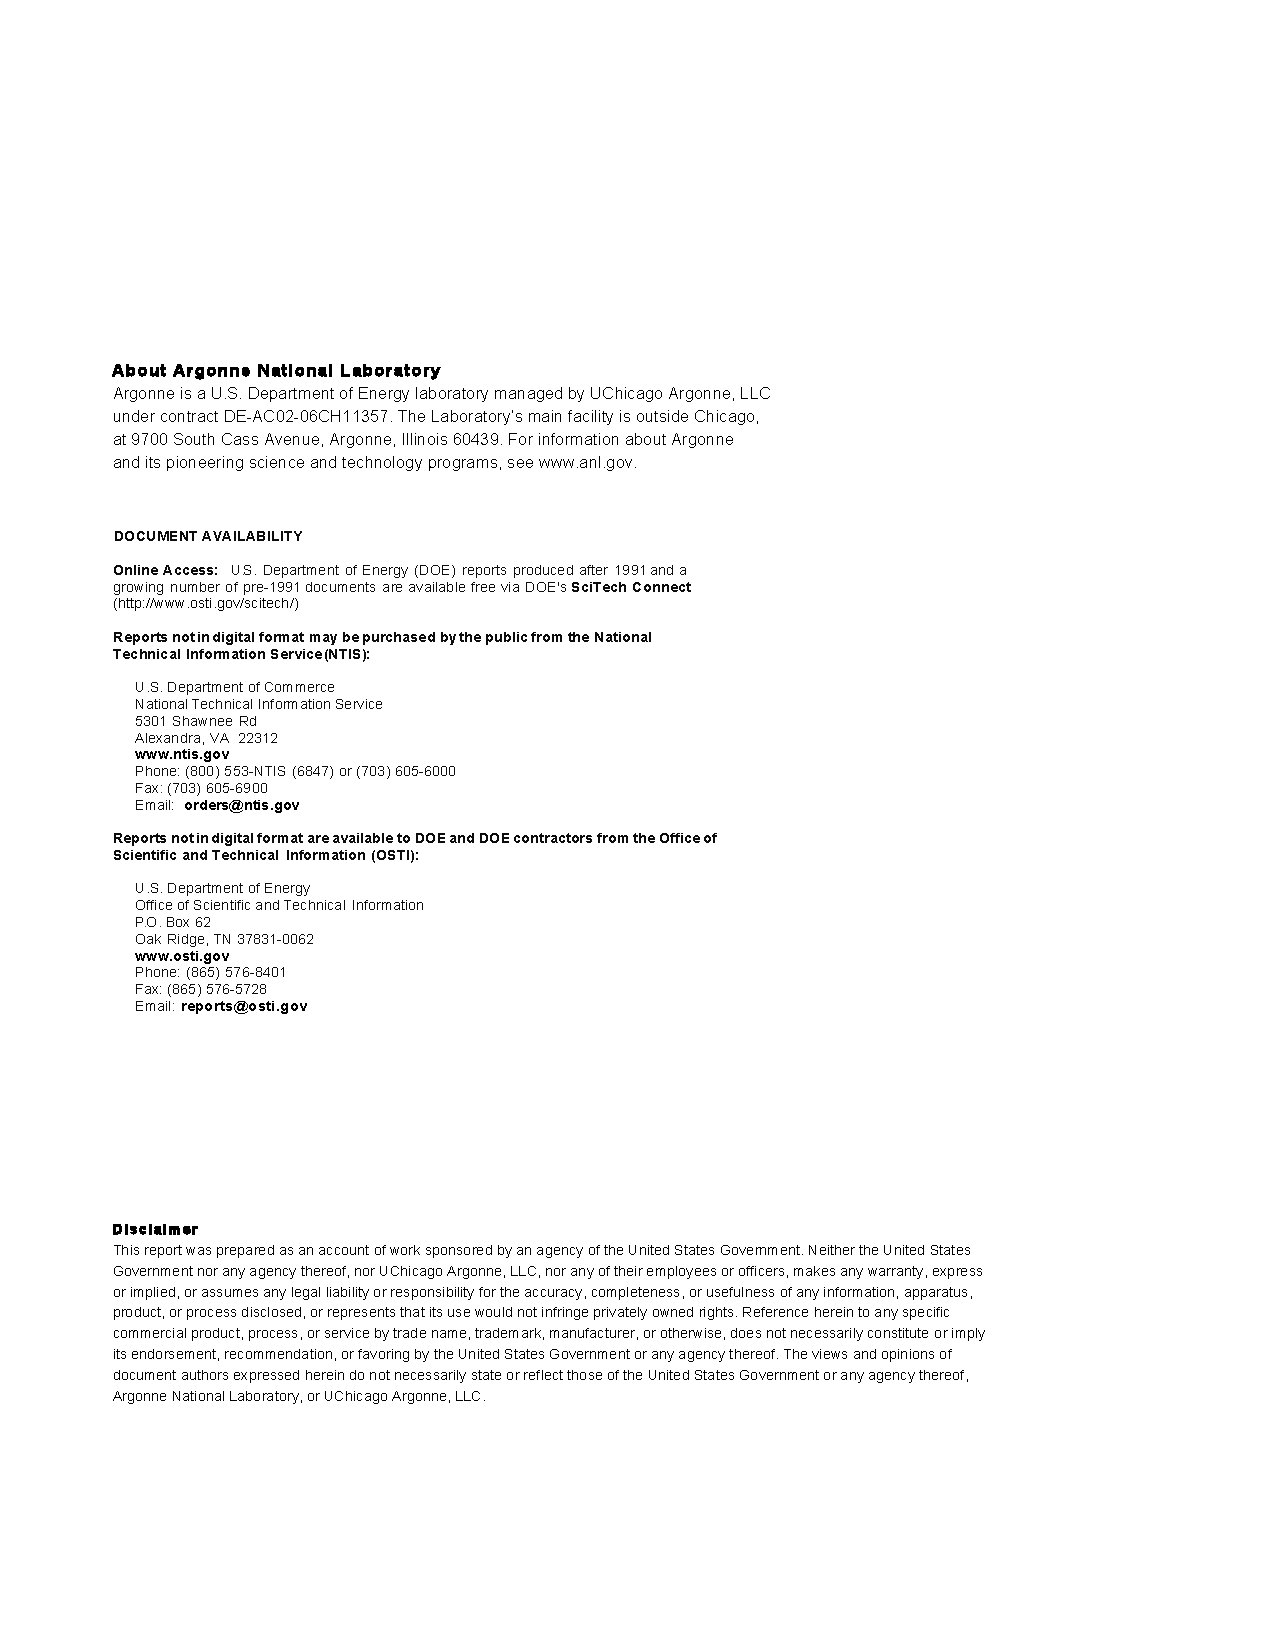
\includegraphics{ArgonneReportTemplatePage2}}
\newpage

\hfill {\large {\bf ANL-95/11 Rev 3.6}}

\vspace*{3in}
\noindent {\LARGE{\bf PETSc Users Manual}}
\vspace*{8pt}
\hrule
\vspace*{8pt}
\noindent {\Large{\it Revision 3.6}}

\vspace*{1in}
\noindent Prepared by \\
S. Balay, S. Abhyankar, M. Adams, J. Brown, P. Brune, K. Buschelman, L. Dalcin, V. Eijkhout, W. Gropp, D. Karpeyev,
D. Kaushik, M. Knepley, L. Curfman McInnes, K. Rupp, B. Smith, S. Zampini, and H. Zhang
Mathematics and Computer Science Division, Argonne National Laboratory

\vspace*{30pt}
\noindent June 2015

\vspace*{20pt}
\noindent This work was supported by the Office of Advanced Scientific Computing Research, \\
Office of Science, U.S. Department of Energy, under Contract DE-AC02-06CH11357.


\cleardoublepage
%\pagestyle{plain}
\pagestyle{fancy}
\vspace{1in}
\date{\today}

% Abstract for users manual
\addcontentsline{toc}{chapter}{Abstract}
% Abstract for TAO Users Manual

\addcontentsline{toc}{chapter}{Preface}
\section*{Preface}

The Toolkit for Advanced Optimization (TAO) focuses on the development
of algorithms and software for the solution of large-scale optimization 
problems on high-performance architectures.  Areas of interest include 
unconstrained and bound-constrained optimization, nonlinear least squares 
problems, optimization problems with partial differential equation 
constraints, and variational inequalities and complementarity 
constraints.

The development of TAO was motivated by the scattered support for
parallel computations and the lack of reuse of external toolkits in
current optimization software.  Our aim is to produce high-quality 
optimization software for computing environments ranging from 
workstations and laptops to massively parallel high-performance 
architectures.  Our design decisions are strongly motivated by 
the challenges inherent in the use of large-scale distributed 
memory architectures and the reality of working with large, 
often poorly structured legacy codes for specific 
applications.

%%% Local Variables: 
%%% mode: latex
%%% TeX-master: "manual_tex"
%%% End: 



\cleardoublepage


% ---------------------------------------------------------------------------
%

\medskip\medskip

\noindent {\bf Getting Information on PETSc:}

\medskip


\noindent {\bf On-line:}
\begin{list}{$\bullet$}
{
\setlength{\itemsep}{-.020in}
\setlength{\topsep}{0in}
\setlength{\partopsep}{0in}
}
\item Manual pages--example usage
\href{index.html}{docs/index.html}  or
\href{http://www.mcs.anl.gov/petsc/documentation}{http://www.mcs.anl.gov/petsc/documentation}
\item Installing PETSc
\href{http://www.mcs.anl.gov/petsc/documentation/installation.html}{http://www.mcs.anl.gov/petsc/documentation/installation.html}
\end{list}

\medskip
\noindent {\bf In this manual:}
\begin{list}{$\bullet$}
{
\setlength{\itemsep}{-.02in}
\setlength{\topsep}{.02in}
\setlength{\partopsep}{0in}
}
\item Basic introduction, page \pageref{sec_gettingstarted}
\item Assembling vectors, page \pageref{sec_vecbasic}; and matrices, \pageref{chapter_matrices}
\item Linear solvers, page \pageref{ch_ksp}
\item Nonlinear solvers, page \pageref{chapter_snes}
\item Timestepping (ODE) solvers, page \pageref{chapter_ts}
\item Index, page \pageref{ch_index}
\end{list}

% ---------------------------------------------------------------------------


\medskip \medskip

\cleardoublepage

% Acknowledgements for users manual
% Acknowledgements for PETSc Users Manual
%
%   this information is a DUPLICATE of misc/acknwldg.htm
%                MAKE SURE THEY MATCH!!!
%
\noindent {\bf Acknowledgments:}

\medskip \medskip \noindent
We thank all PETSc users for their many suggestions, bug reports, and
encouragement.  We especially thank David Keyes
for his valuable comments on the source code,
functionality, and documentation for PETSc.


\vspace{.3in}
\noindent
Some of the source code and utilities in PETSc
have been written by
\begin{itemize}
  \item Asbjorn Hoiland Aarrestad - the explicit Runge-Kutta implementations;
  \item G. Anciaux and J. Roman - the interfaces to the partitioning packages PTScotch, Chaco, and Party;
  \item Allison Baker - the flexible GMRES code and LGMRES;
  \item Chad Carroll - Win32 graphics;
  \item Ethan Coon - the PetscBag and many bug fixes;
  \item Cameron Cooper - portions of the VecScatter routines;
  \item Patrick Farrell - nleqerr line search for SNES
  \item Paulo Goldfeld - balancing Neumann-Neumann preconditioner;
  \item Matt Hille;
  \item Joel Malard - the BICGStab(l) implementation;
  \item Paul Mullowney, enhancements to portions of the Nvidia GPU interface;
  \item Dave May - the GCR implementation
  \item Peter Mell - portions of the DA routines;
  \item Richard Mills - the AIJPERM matrix format for the Cray X1 and universal F90 array interface;
  \item Victor Minden - the NVidia GPU interface;
  \item Todd Munson - the LUSOL (sparse solver in MINOS) interface and several Krylov methods;
  \item Adam Powell - the PETSc Debian package,
  \item Robert Scheichl - the MINRES implementation,
  \item Kerry Stevens - the pthread based Vec and Mat classes plus the various thread pools
  \item Karen Toonen - designed and implemented much of the PETSc web pages,
  \item Desire Nuentsa Wakam - the deflated GMRES implementation,
  \item Liyang Xu - the interface to PVODE (now Sundials/CVODE).
\end{itemize}

\vspace{.3in}
\noindent
PETSc source code contains modfied routines from the following public domain software packages
\begin{itemize}
  \item LINPACK -    dense matrix factorization and solve; converted to C using {\tt f2c} and then
                     hand-optimized for small matrix sizes, for block matrix data structures;
  \item MINPACK -    see page \pageref{sec_fdmatrix}, sequential matrix coloring routines for finite difference Jacobian
                     evaluations; converted to C using {\tt f2c};
  \item SPARSPAK -   see page \pageref{sec_factorization}, matrix reordering routines, converted to C using {\tt f2c};
  \item libtfs     - the efficient, parallel direct solver developed by Henry Tufo and Paul Fischer for the direct solution of a coarse grid problem
                     (a linear system with very few degrees of freedom per processor).
\end{itemize}


\vspace{.3in}
\noindent
PETSc interfaces to the following external software:
\begin{itemize}
  \item ADIFOR -  automatic differentiation for the computation of sparse Jacobians,\\
                     \href{http://www.mcs.anl.gov/adifor}{http://www.mcs.anl.gov/adifor},
  \item BLAS and LAPACK - numerical linear algebra,
  \item Chaco -     A graph partitioning package, \href{ http://www.cs.sandia.gov/CRF/chac.html}{ http://www.cs.sandia.gov/CRF/chac.html}
  \item ESSL -         IBM's math library for fast sparse direct LU factorization,
  \item Elemental -  Jack Poulson's parallel dense matrix solver package,
  \item hypre -    the LLNL preconditioner library, \href{http://www.llnl.gov/CASC/hypre}{http://www.llnl.gov/CASC/hypre}
  \item LUSOL -       sparse LU factorization code (part of MINOS) developed by Michael Saunders,
                      Systems Optimization Laboratory, Stanford University,
                     \href{http://www.sbsi-sol-optimize.com/}{http://www.sbsi-sol-optimize.com/},
  \item Mathematica -  see page \pageref{ch_mathematica},
  \item MATLAB -      see page \pageref{ch_matlab},
  \item MUMPS -      see page \pageref{sec_externalsol}, MUltifrontal Massively Parallel sparse direct Solver developed by Patrick Amestoy,
                     Iain Duff, Jacko Koster, and Jean-Yves L'Excellent, \\
                     \href{http://www.enseeiht.fr/lima/apo/MUMPS/credits.html}{http://www.enseeiht.fr/lima/apo/MUMPS/credits.html},
  \item Metis/ParMeTiS - see page \pageref{sec_partitioning}, parallel graph partitioner,
                     \href{http://www-users.cs.umn.edu/~karypis/metis/}{http://www-users.cs.umn.edu/~karypis/metis/},
  \item Party -     A graph partitioning package, \\ 
               \href{http://www2.cs.uni-paderborn.de/cs/ag-monien/PERSONAL/ROBSY/party.html}{http://www2.cs.uni-paderborn.de/cs/ag-monien/PERSONAL/ROBSY/party.html},
  \item PaStiX -     Parallel LU and Cholesky solvers,
  \item PTScotch -    A graph partitioning package, \href{http://www.labri.fr/Perso/~pelegrin/scotch/}{http://www.labri.fr/Perso/~pelegrin/scotch/}
  \item SPAI -        for parallel sparse approximate inverse preconditiong,
  \item SparseSuite - see page \pageref{sec_externalsol},  developed by Timothy A. Davis,
                    \href{http://faculty.cse.tamu.edu/davis/suitesparse.html}{http://faculty.cse.tamu.edu/davis/suitesparse.html}.
  \item Sundial/CVODE - see page \pageref{sec_sundials}, parallel ODE integrator,
                     \href{http://www.llnl.gov/CASC/sundials/}{http://www.llnl.gov/CASC/sundials/},
  \item SuperLU and SuperLU\_Dist - see page \pageref{sec_externalsol},
                    the efficient sparse LU codes developed by Jim Demmel,  Xiaoye S. Li, and John Gilbert,
                    \href{http://crd-legacy.lbl.gov/~xiaoye/SuperLU}{http://crd-legacy.lbl.gov/~xiaoye/SuperLU},
  \item Triangle and Tetgen - mesh generation packages,
  \item Trilinos/ML - Sandia's main multigrid preconditioning package, \href{http://software.sandia.gov/trilinos/}{http://software.sandia.gov/trilinos/},
  \item Zoltan - graph partitioners from Sandia National Laboratory
\end{itemize}
These are all optional packages and do not need to be installed to use PETSc.

PETSc software is developed and maintained using
\begin{itemize}
\item Emacs editor
\item \href{http://git-scm.com/}{Git} revision control system
\item Python
\end{itemize}

PETSc documentation has been generated using
\begin{itemize}
\item the \href{http://www.cs.uiuc.edu/~wgropp/projects/software/sowing/index.htm}{text processing tools} developed by Bill Gropp
\item c2html
\item pdflatex
\item python
\end{itemize}



% Blank page makes double sided printout look bettter.

\cleardoublepage

\tableofcontents

% --------------------------------------------------------------------
%                            PART 1
% --------------------------------------------------------------------
\cleardoublepage
\part{Introduction to PETSc}
\label{part_intro}
\cleardoublepage
\chapter{Getting Started}
\input{part1tmp.tex}

% --------------------------------------------------------------------
%                            PART 2
% --------------------------------------------------------------------
\cleardoublepage
\part{Programming with PETSc}
\label{part_usage}
\input{part2tmp.tex}


%------------------------------------------------------------------


\cleardoublepage
\bibliographystyle{plain}
\addtocounter{chapter}{1}
\addcontentsline{toc}{chapter}{Bibliography}
\label{sec:bib}
\bibliography{../petsc,../petscapp}

\pagestyle{empty}
\begin{figure*}[hbt]
\centerline{
\includegraphics{ArgonneReportTemplateLastPage.pdf}}
\caption{}
\end{figure*}

\end{document}
